\documentclass[14pt]{beamer}
\title[COJ:Java:03]{COJ :: Polymorphism}
\author[TS]{TalentSprint}
\institute[L\&D]{Licensed To Skill}
\date{Version 1.0.4}
\usefonttheme{serif}
\usecolortheme{orchid}
\usepackage{bookman}
\usepackage{hyperref}
\usepackage[T1]{fontenc}
\usepackage{graphicx}
\graphicspath{{../../Images/}}
\usepackage{listings}
\beamertemplateballitem
\usebackgroundtemplate{
\includegraphics[width=\paperwidth]{TS-Logo.jpg}}
\lstset{language=Java,numbers=left, numberstyle=\tiny, numbersep=10pt, showstringspaces=false, breaklines=true,keepspaces=true, columns=flexible}
\begin{document}

\begin{frame}
  \titlepage
\end{frame}

\begin{frame}{Learning Objectives}
By the end of this session, you will be able to:
  \begin{itemize}

  \item Polymorphism and Overriding

  \end{itemize}
\end{frame}

\begin{frame}[fragile]{Polymorphism}
Exercise 1
\begin{lstlisting}[numbers=none, basicstyle=\tiny]
Create the following Employee, Manager, Clerk, SalesPerson classes in java.

- Employee 
Instance variables : name, salaryBasic, HRAPer, DAPer, PT. 
Methods : computePayroll()

- Manager ( a sub class of Employee)
  Instance variable :  projectAllowance 
  Methods : computePayroll()

- Clerk ( a sub class of Employee)
  Instance variable : int typingSpeed , int typingAccuracy
  Methods : computePayroll()

- SalesPerson ( a sub class of Employee)
  Instance variable :  noOfTargetsCompleted, perkTarget
  Methods : computePayroll()
\end{lstlisting}

\begin{lstlisting}[numbers=none, basicstyle=\tiny]
Create appropriate constructors for all the classes.

Create a class with main and add a displaySalary()  method which takes one parameter of type employee and complete the application by using the computePayroll() method in displaySalary() method.
\end{lstlisting}
\end{frame}



\begin{frame}{Polymorphism}
Polymorphism is a concept where a single name may denote objects of different classes that are related by some common base class. 

Polymorphism is the ability to create an attribute, a method, or an object that has more than one form.
\end{frame}


\begin{frame}{Polymorphism}
 \begin{itemize}
  \item A polymorphic reference variable can refer to different types of objects at different times
  \item In java every reference can be polymorphic except of references to base types and final classes
  \item It is the type of the object being referenced, not the reference type, that determines which method is invoked
  \item Polymorphic references are therefore resolved at run-time, not during compilation; this is called dynamic binding
   \end{itemize}

\end{frame}

\begin{frame}[fragile]{Polymorphism}
 \begin{block}{Example: Overriding Methods }
\begin{lstlisting}[numbers=none, basicstyle=\tiny]
class Employee {                                class Manager extends Employee {
    int empId;                                      double projAllowance;
    String name;                                    Manager(int id,String name double pAllowance) {
    Employee(int id,String eName) {                     super(id, name);
        empId = id;                                     projAllowance = pAllowance;
        name = eName                                }
    }                                               void display() {
    void display() {                                    System.out.println("id, name and pAllowance:" + id +
        System.out.println("id and name: "                        " "+ name + " " + projAllowance);
               + id + " " + name);                  }
    }                                           }
}
  \end{lstlisting}
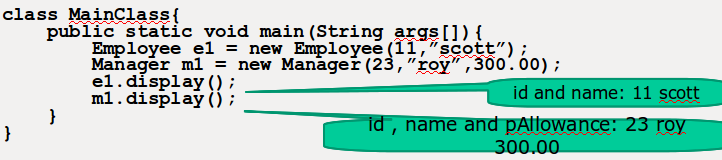
\includegraphics[scale=.42]{overriding-main-class.png}
 \end{block}
\end{frame}


\begin{frame}{Polymorphism}
 How does it work?
 \vspace{1pc}
 
 What happened to the \textbf{display()} method of super class while calling \textbf{m1.display()}
 \vspace{1pc}
 
 Can we access the \textbf{display()} method of the super class Employee from sub class Manager ?
\end{frame}

\begin{frame}[fragile]{Polymorphism}
 Overriding
 
 \begin{figure}[H]
\begin{minipage}[l]{0.5\linewidth}
\begin{lstlisting}[numbers=none, basicstyle=\tiny]

class  One {
    int x1 = 10;
    public int m1(int x1) {
        return x1 * x1;
    }
}

class Two {
    int x2 = 20;
    public int m2() {
        return x2;
    }
}

class MainClass {
  pubic static void main(String args[]) {
      One one = new One();
      Two two = new Two();
    }
}
\end{lstlisting}

\end{minipage}
\quad
\begin{minipage}[c]{0.3\textwidth}
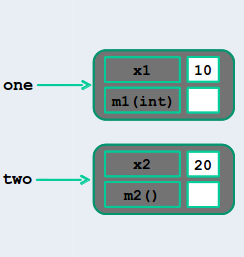
\includegraphics[scale=.4]{poly-program.png}

\end{minipage}
\end{figure}
\end{frame}

\begin{frame}[fragile]{Polymorphism}
 Overriding
 
 \begin{figure}[H]
\begin{minipage}[l]{0.5\linewidth}
\begin{lstlisting}[numbers=none, basicstyle=\tiny, linebackgroundcolor={\ifnum\value{lstnumber}=3\color{green}\fi}]

class  SuperClass {
    int x1 = 10;
    public int m1(int value) {
        return value * value;
    }
}
class SubClass extends SuperClass {
    int x2 = 20;
    public int m2(){
        return x2;
    }
}
class MainClass {
    pubic static void main(String args[]) {
        SuperClass one = new SuperClass();
        SubClass two = new SubClass();
    }
}
\end{lstlisting}

\end{minipage}
\quad
\begin{minipage}[c]{0.3\textwidth}
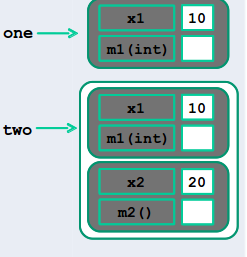
\includegraphics[scale=.4]{poly-override.png}

\end{minipage}
\end{figure}
\end{frame}


\begin{frame}[fragile]{Polymorphism}
 Overriding
 
 \begin{figure}[H]
\begin{minipage}[l]{0.5\linewidth}
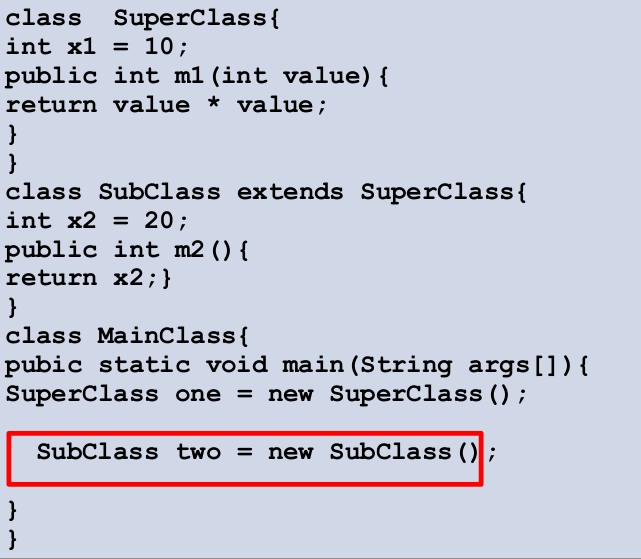
\includegraphics[scale=.2]{polyoverride3.png}

\end{minipage}
\quad
\begin{minipage}[c]{0.3\textwidth}
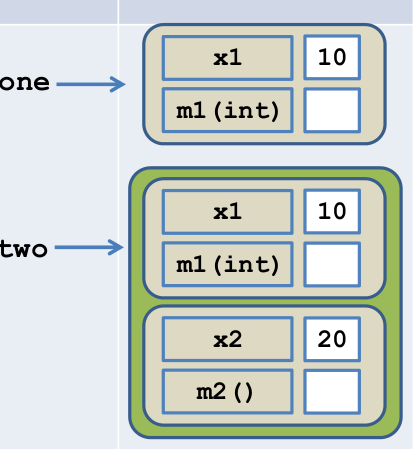
\includegraphics[scale=.2]{polyoverride4.png}

\end{minipage}
\end{figure}
\end{frame}

\begin{frame}[fragile]{Polymorphism}
 Overriding
 
 \begin{figure}[H]
\begin{minipage}[l]{0.5\linewidth}
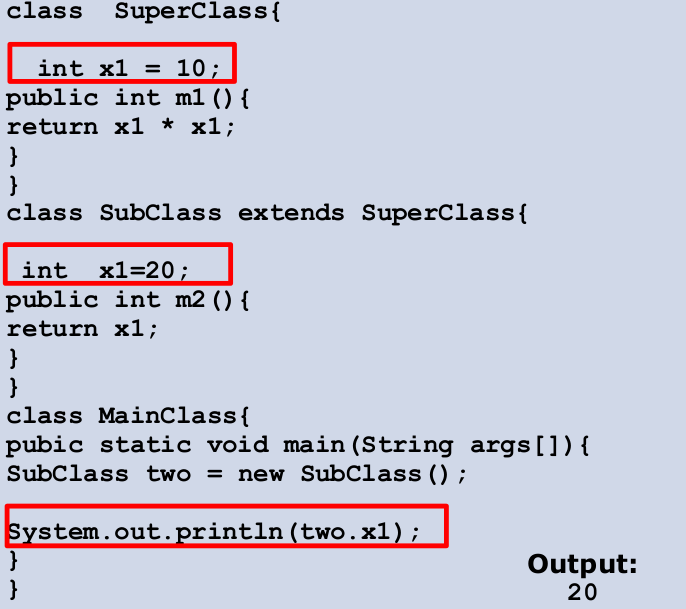
\includegraphics[scale=.2]{polyoverride1.png}

\end{minipage}
\quad
\begin{minipage}[c]{0.3\textwidth}
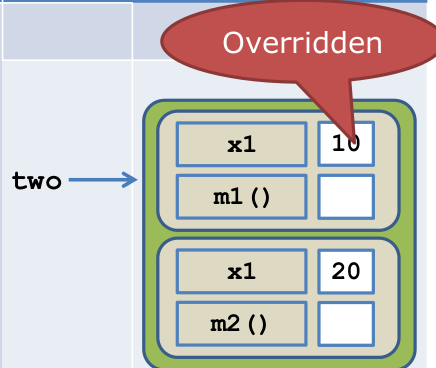
\includegraphics[scale=.2]{polyoverride2.png}

\end{minipage}
\end{figure}
\end{frame}

\begin{frame}[fragile]{Polymorphism}
 Overriding
 
 \begin{figure}[H]
\begin{minipage}[l]{0.5\linewidth}
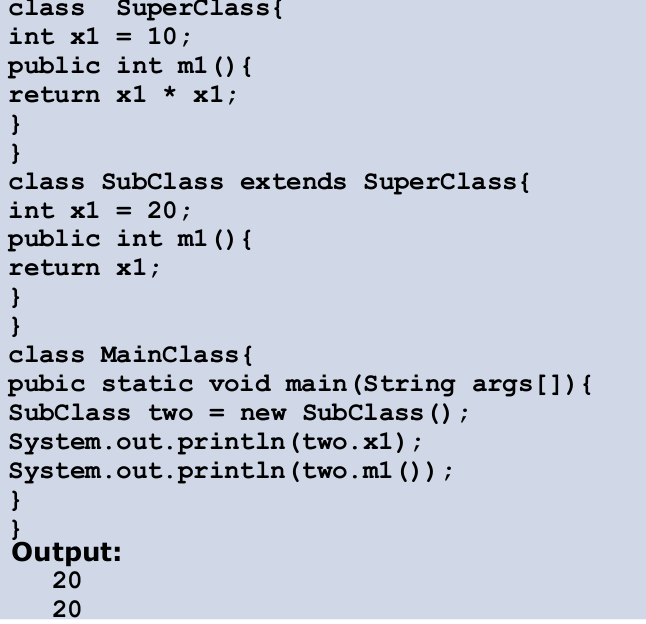
\includegraphics[scale=.2]{polyoverride5.png}

\end{minipage}
\quad
\begin{minipage}[c]{0.3\textwidth}
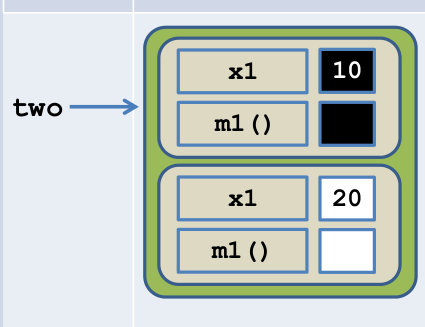
\includegraphics[scale=.2]{polyoverride6.png}

\end{minipage}
\end{figure}
\end{frame}

\begin{frame}[fragile]{Overloading Methods}
\begin{itemize}
\item When a method of a sub-class has the same name and type as a method of the super-class, we say that this method is overridden.
\item Overriding method has the same name, number and type of parameters, and return type as the method it overrides.
\end{itemize}
\end{frame}

\begin{frame}[fragile]{Overriding}
 
 
 \begin{figure}[H]
\begin{minipage}[l]{0.5\linewidth}
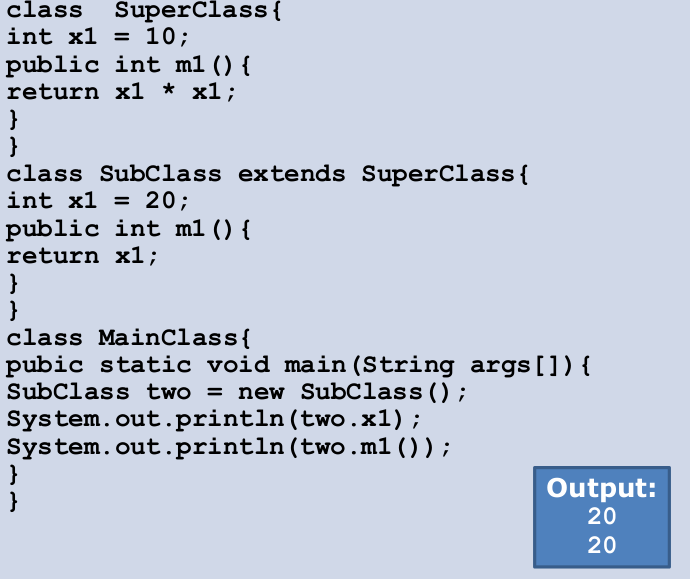
\includegraphics[scale=.2]{polyoverride7.png}

\end{minipage}
\quad
\begin{minipage}[c]{0.3\textwidth}
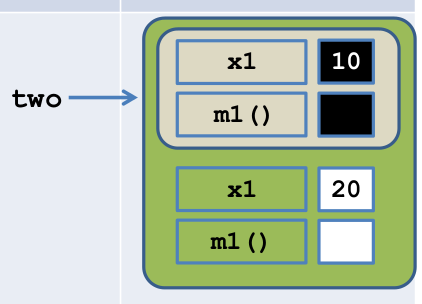
\includegraphics[scale=.2]{polyoverride8.png}

\end{minipage}
\end{figure}
\end{frame}

\begin{frame}[fragile]{Overriding}
 
 
 \begin{figure}[H]
\begin{minipage}[l]{0.5\linewidth}
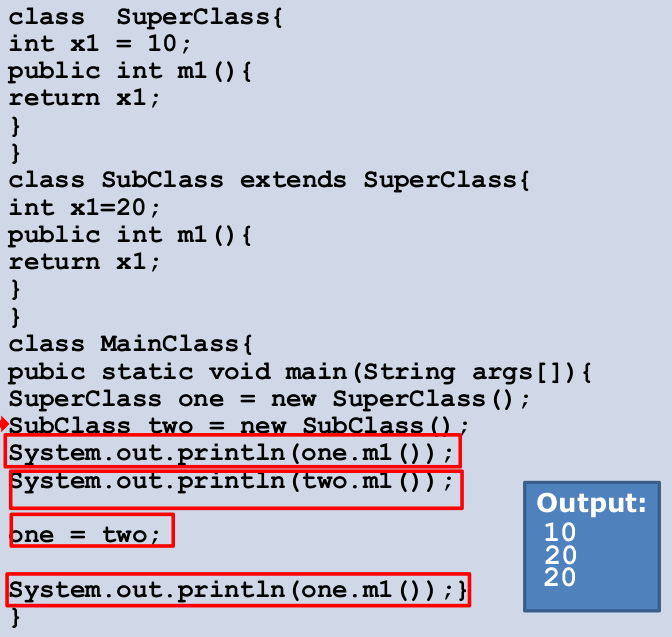
\includegraphics[scale=.2]{polyoverride9.png}

\end{minipage}
\quad
\begin{minipage}[c]{0.3\textwidth}
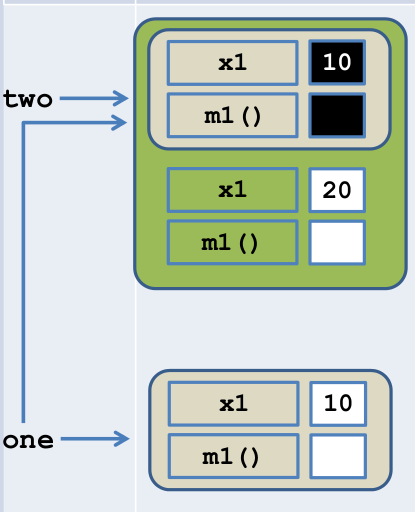
\includegraphics[scale=.2]{polyoverride10.png}

\end{minipage}
\end{figure}
\end{frame}

\begin{frame}{Introduction To Overloading}
\begin{itemize}
\item The ability to allow different methods or constructors of a class to share the same name
\item Always remember that overloaded methods have the following properties:
\begin{itemize}
\item The same method name
\item type of parameters or number of parameters or order of parameters should be different.
\item Return types can be different or same
\end{itemize}
\end{itemize}
\end{frame}

\begin{frame}{Introduction To Overloading}
\begin{itemize}
\item A method can be overloaded in the same class or in a subclass.
\item Access modifier can be different.
\end{itemize}
\end{frame}

\begin{frame}{Overloading A Method Name}
\begin{center}
Same Method Name Means (does) different things in different circumstances
\end{center}
\end{frame}


\begin{frame}{Method Overloading}
\begin{center}
    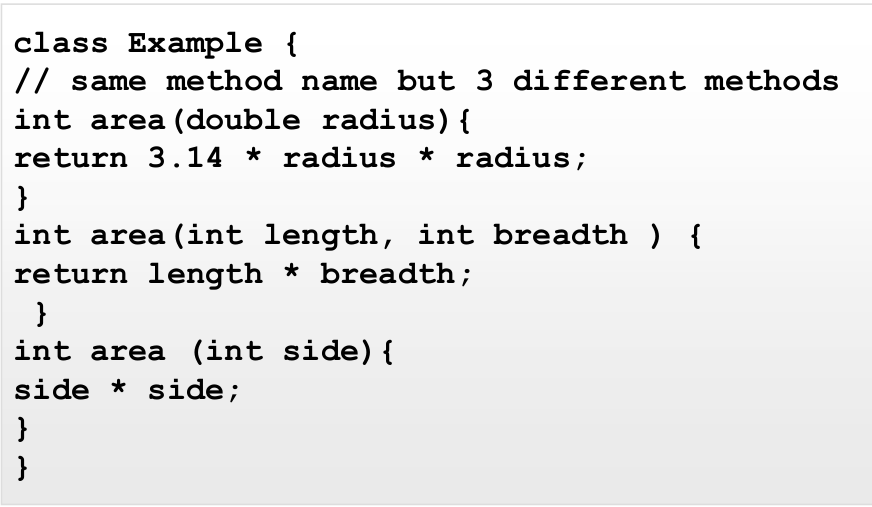
\includegraphics[scale=0.3]{overload1.png}
  \end{center}
 \end{frame}

\begin{frame}{Polymorphism}
\begin{center}
    
\includegraphics[scale=0.5]{qa.png}
  \end{center}
\end{frame}

\end{document}


